\documentclass[a0,landscape]{a0poster}

\usepackage{multicol}
\columnsep=100pt
\columnseprule=3pt

\usepackage[svgnames]{xcolor}

\usepackage{times}

\usepackage{graphicx}
\graphicspath{{figures/}}
\usepackage{booktabs}
\usepackage[font=small,labelfont=bf]{caption}
\usepackage{amsfonts, amsmath, amsthm, amssymb}
\usepackage{wrapfig}

\begin{document}

\begin{minipage}[b]{0.55\linewidth}
\veryHuge \color{NavyBlue} \textbf{An IMS-based AS/MRFC Model for IVR Services} \color{Black}\\
\Huge\textit{Research \& Implementation}\\[1cm]
\LARGE \textbf{Youzheng Chen, Baozhong Cheng, etc.}\\
\LARGE Beijing University of Posts and Telecommunications\\
\end{minipage}
%
\begin{minipage}[b]{0.25\linewidth}
\color{DarkSlateGray}\Large \textbf{Contact Information:}\\
School of Software Engineering\\
Beijing Univ. Post. \& Telecom.\\
\#10 Xitucheng Rd, Haidian Dist.\\
Beijing 100876 China\\\\
Phone: (+86)-10-5882-8040\\
Email: \texttt{bzcheng@bupt.edu.cn}\\
\end{minipage}
%
\begin{minipage}[b]{0.19\linewidth}

\includegraphics[width=21cm]{logo.eps}
\end{minipage}

\vspace{1cm}

\begin{multicols}{4}

\color{SaddleBrown}

\section{Introduction}

\Large Proposed by 3GPP, IMS is a service development architecture for the NGN. Interactive Voice Response (IVR) is one of the important techniques to develop new self-services in IMS network for reducing IMS running cost. However, most of the IVR systems nowadays are designed for a small scale, so they may not be scalable and flexible enough for the requirement of IMS network. 

In this research work, a new solution of IVR Function in IMS area is proposed.
\begin{itemize}
\item Propose an architecture of value-added business with high scalability and openness for business adaptation;
\item Develop and implement a prototype to prove the feasibility and compatibility of this solution;
\end{itemize}

\color{DarkSlateGray}

\section{Problem Analysis}

In order to integrate IVR system into IMS network as a value-added service, the architecture of IMS defined by 3GPP is referred and improved for the specific requirement in this area. 

For the requirement of providing separated services to different subscribers, the user preferences should be recorded in this system. We introduce Subscriber Policy for retrieving specific preference when a call is incoming. In a higher level of abstraction, business logic is defined as Speech Script in this research.

Speech Script database is defined as Speech Script Server. The script can be static, which is stored in file system, or it can also be dynamic. In the second case, the script can be dynamically generated as JavaServer Pages (JSP) or Servlet according to the business logic and the user preferences.

\section{Design and Inplementation}

In order to solve this problem, we have consulted the Technical Report of 3GPP. It has proposed a solution for functional split between the AS and MRFC on conference focus. Such solution can also be applied to our situation with necessary modifications. In this way, we propose our solution of IVR Function (shown in Figure 1). The terminology and concepts are still reused from IETF standards.

\begin{center}\vspace{1cm}
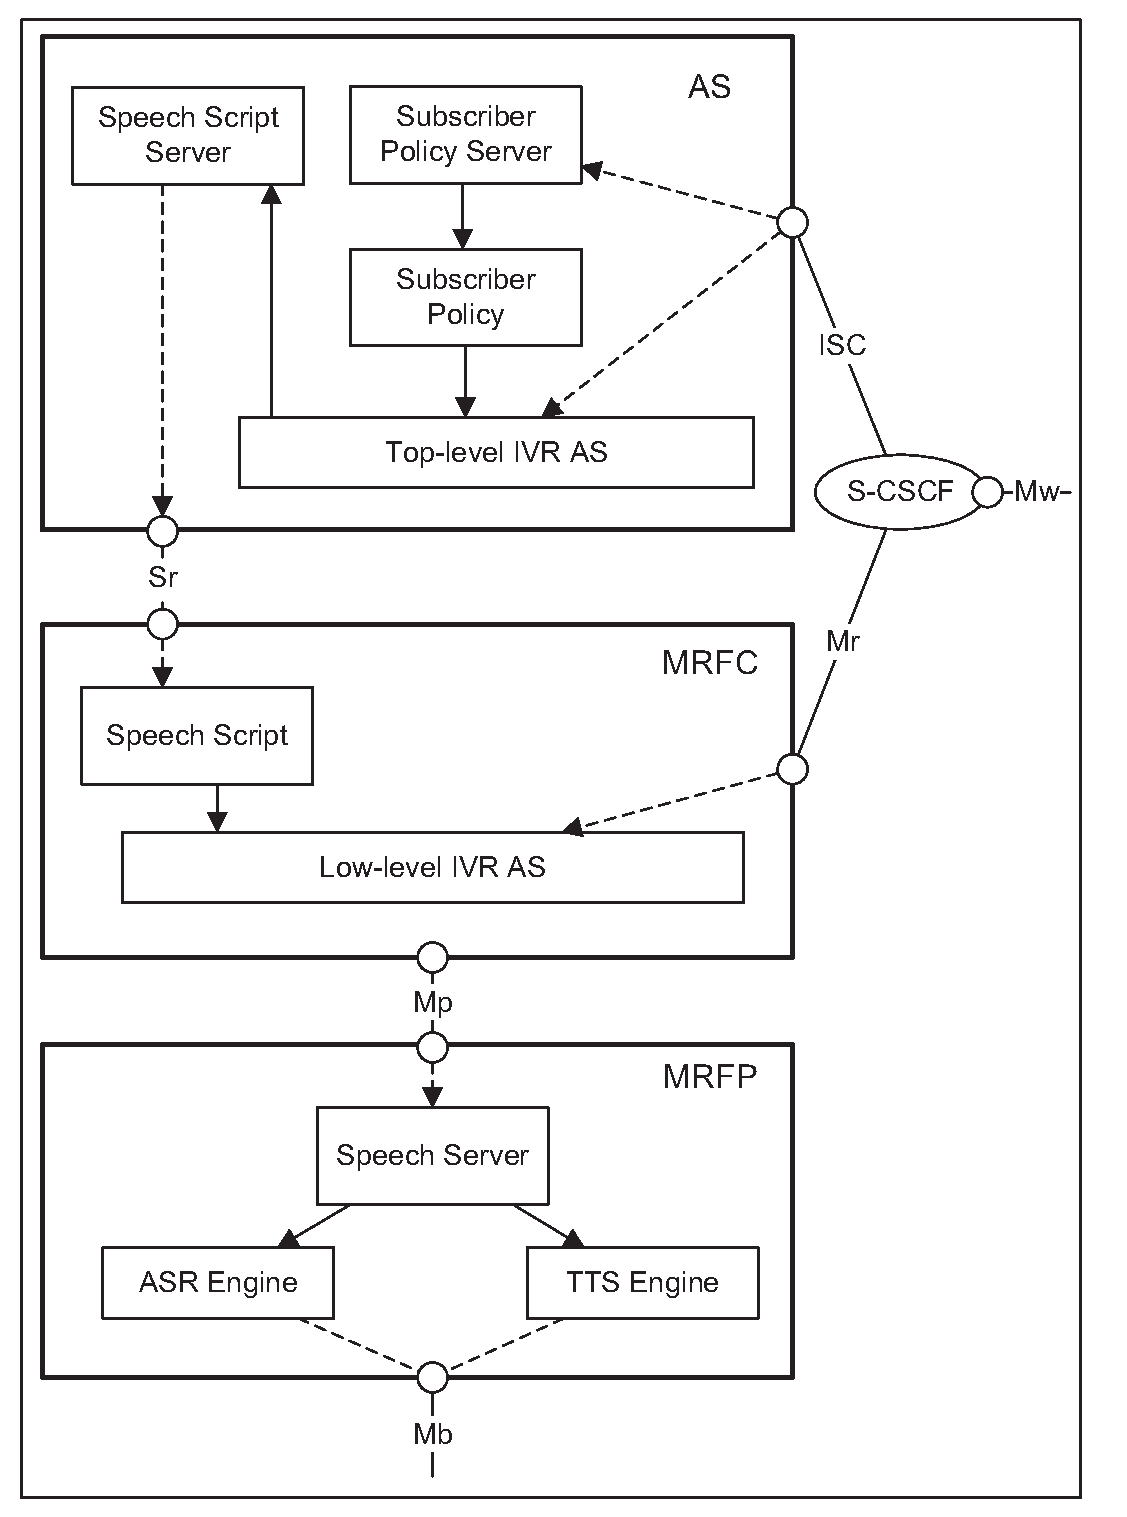
\includegraphics[width=0.7\linewidth]{split.eps}
\captionof{figure}{\color{Green} Our Solution of IVR Function.}
\end{center}\vspace{1cm}

The collocated AS/MRFC model is split between two sets of servers: Top-level IVR AS and Low-level IVR AS. The Top-level IVR AS, which maintains the role of IMS AS, is used to handle the jobs related to the preferences of subscribers, while the Low-level IVR AS, which plays the role of IMS MRFC, is used to deal with the speech application logic assigned by the top-level ones.

In details, the Top-level IVR AS, is used to
\begin{enumerate}
\item Implement the Subscriber Policy Server, for identifying the incoming call and present the related user preference. And the user data can be subscribed and modified by the end-users.
\item Generate the related business logic through Speech Script Server accordingly and send to the Low-level IVR AS.
\item Maintain user dialogs and redirect or transfer dialogs according to the instruction of the Low-level IVR AS.
\item Might support billing and charging.
\end{enumerate}

And the Low-level IVR AS, is used to
\begin{enumerate}
\item Load and execute the Speech Script, such as VoiceXML, CCXML, and SCXML.
\item Control the speech-related logic on MRFP, and the dialog manipulation on AS.
\end{enumerate}

According to the design described above, a prototype project is designed and implemented in order to prove the feasibility. As Figure 2 depicts, this solution can be viewed as three parts: IMS Client, IMS Core and IMS Services.

\begin{center}\vspace{1cm}
\includegraphics[width=0.6\linewidth]{Architecture.eps}
\captionof{figure}{\color{Green} The Architecture of the Solution.}
\end{center}\vspace{1cm}

\begin{center}\vspace{1cm}
\centering
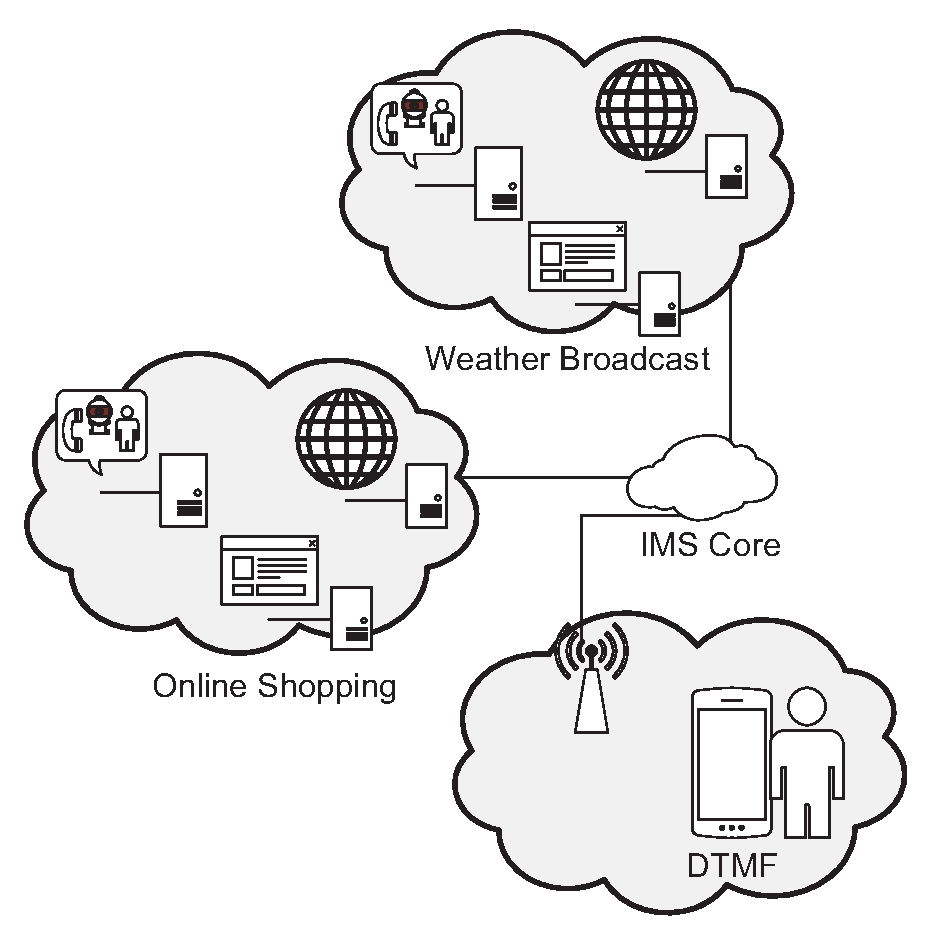
\includegraphics[width=0.4\linewidth]{scenario_a.eps}
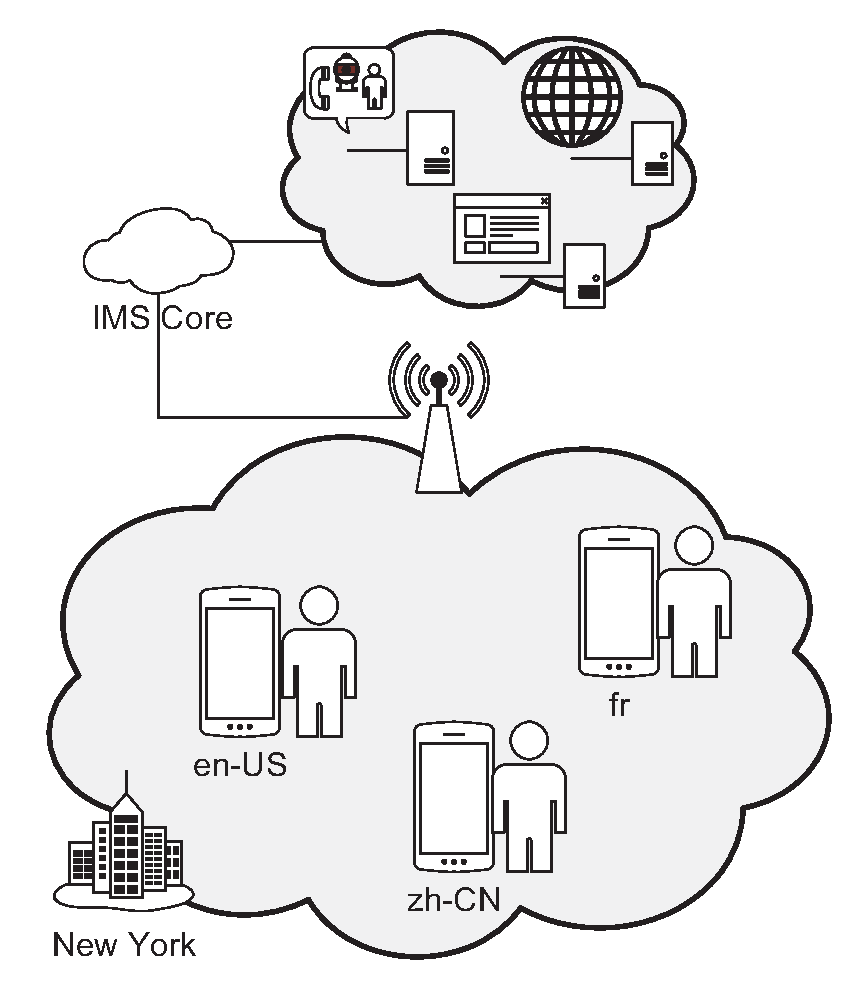
\includegraphics[width=0.4\linewidth]{scenario_b.eps}
\captionof{figure}{\color{Green} The Application Scenarios.}
\end{center}\vspace{1cm}

For the application of this solution, we present two scenarios, which significantly show the improvement of the user experience and the reduction of the running costs brought by our solution. Figure 3 depicts two of these application scenarios.

\color{SaddleBrown}

\section{Conclusions}

In this research, the functional split between AS and MRFC in IVR Function provides a new solution to IVR Function in IMS network area, which not only brings telecommunication service providers an opportunity to integrate most of the IVR services through customized speech scripts, but also improves the user experience for subscribers through shared user preference information among different services and different providers.

\color{DarkSlateGray}

\section*{Acknowledgements}

The authors would like to thank Kun Li for his valuable advice on architecture design and implementation. And thank Hongye Qi for his contribution to functional requirement.

\end{multicols}
\end{document}